\chapter{Experimenty a výsledky} \label{chapter-experimenty}

V této kapitole se podíváme na tři typy experimentů, které s naším systémem
můžeme provádět. Knihovna implementuje několik různých přístupů jak roboty
řídit a jak je vyvíjet pomocí evolučních algoritmů. Následující experimenty
předvedou vzorek z těchto přístupů. 

Cílem všech následujících experimentů je pomocí evolučních algoritmů vyvinout
zvoleného robota tak, aby byl schopný stabilního pohybu v simulovaném prostředí
v předem určeném směru. Každý jedinec začíná svůj simulační běh v prostředí v
počátku na souřadnicích $(0,0)$. V našem experimentu chceme, aby se robot
pohyboval ve směru rostoucí x-ové souřadnice. Kvalita jedinců je pak jednoduše
vypočtena dle následující rovnice:

\begin{equation} \label{fitness_calc}
    fitness = x - 0.5\cdot|y|
\end{equation}
kde $(x,y)$ jsou souřadnice bodu v simulovaném prostředí, do kterého jedinec
dorazil (buď do vypršení limitovaného času na simulaci, nebo do dosažení
podmínky předčasně ukončující simulační běh -- např. pádu robota).

V prvním experimentu v sekci \ref{exp1} si ověříme přirozený předpoklad, že pro
řízení jednoduchých robotů nám stačí základní evoluční algoritmy a pro
složitější roboty (s větším množstvím stupňů volnosti) potřebujeme pokročilé
přístupy. V následujících dvou experimentech v sekci \ref{exp2} popíšeme
experimenty demonstrující možnost evolučního vývoje jak řízení tak morfologie
robotů.

\section{Vývoj řízení robotů} \label{exp1}

V této sekci se zaměříme na vývoj řízení robotů. Řízení robota je systém,
který na základě vstupů z prostředí (senzory robota, čas, atd.) generuje
signály do výkonných prvků robota (typicky motory). 

Průběh vývoje řízení robota je ovlivněn zvoleným agentem, který definuje
genotyp jedinců a určuje, jaké genetické operátory budou při vývoji využívány.
Podrobnější popis agentů se nachází v sekci \ref{imp:gaAgents}.

\begin{figure}[!htb]
    \centering
    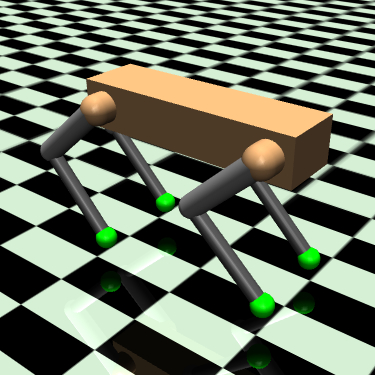
\includegraphics[width=0.4\textwidth]{../img/crop_SpotLike.jpg}
    \caption{Robot \emph{SpotLike}}
    \label{fig:robot:spotlike}
\end{figure}

První pokus se bude snažit vyvinout řízení pro pokročilého robota v projektu
označovaném jako \emph{SpotLike} (na obrázku \ref{fig:robot:spotlike}, blíže
popsaný v implementaci v sekci \ref{imp:robots.Spot}). Jedná se o robota
kráčejícího na čtyřech nohách, kde každá noha má 3 stupně volnosti (tedy celkem
12 pro celého robota). Můžeme ho tedy řadit mezi roboty, u kterých již bude
obtížnější vyvinout stabilní pohyb v určeném směru.

Kráčení, kterého bychom u robotů chtěli dosáhnout, si můžeme představit jako
periodický pohyb, kde každá noha cyklicky opakuje stejné pohyby. Proto se pro
vývoj řízení pokusíme využít agenty, kteří interně podle parametrů generují
periodické hodnoty pro motory robotů. 

\paragraph{Volba parametrů velikosti experimentu}
Pro tento typ experimentu inicializujeme populaci se \textbf{100 jedinci}.
Abychom zjistili, kolik generací je potřeba pro rozumné výsledky, necháme
nejprve proběhnout delší experiment, ve kterém vývoj evolučního algoritmu
poběží po \textbf{500 generací}. Abychom vyloučili vliv náhodné inicializace
populace jedinců v genetickém algoritmu, pro vyhodnocení je celý
běh algoritmu \textbf{20 krát} nezávisle opakován a výsledky prezentujeme
pomocí následujícího typu grafu.

\begin{figure}[!htb]
    \centering
    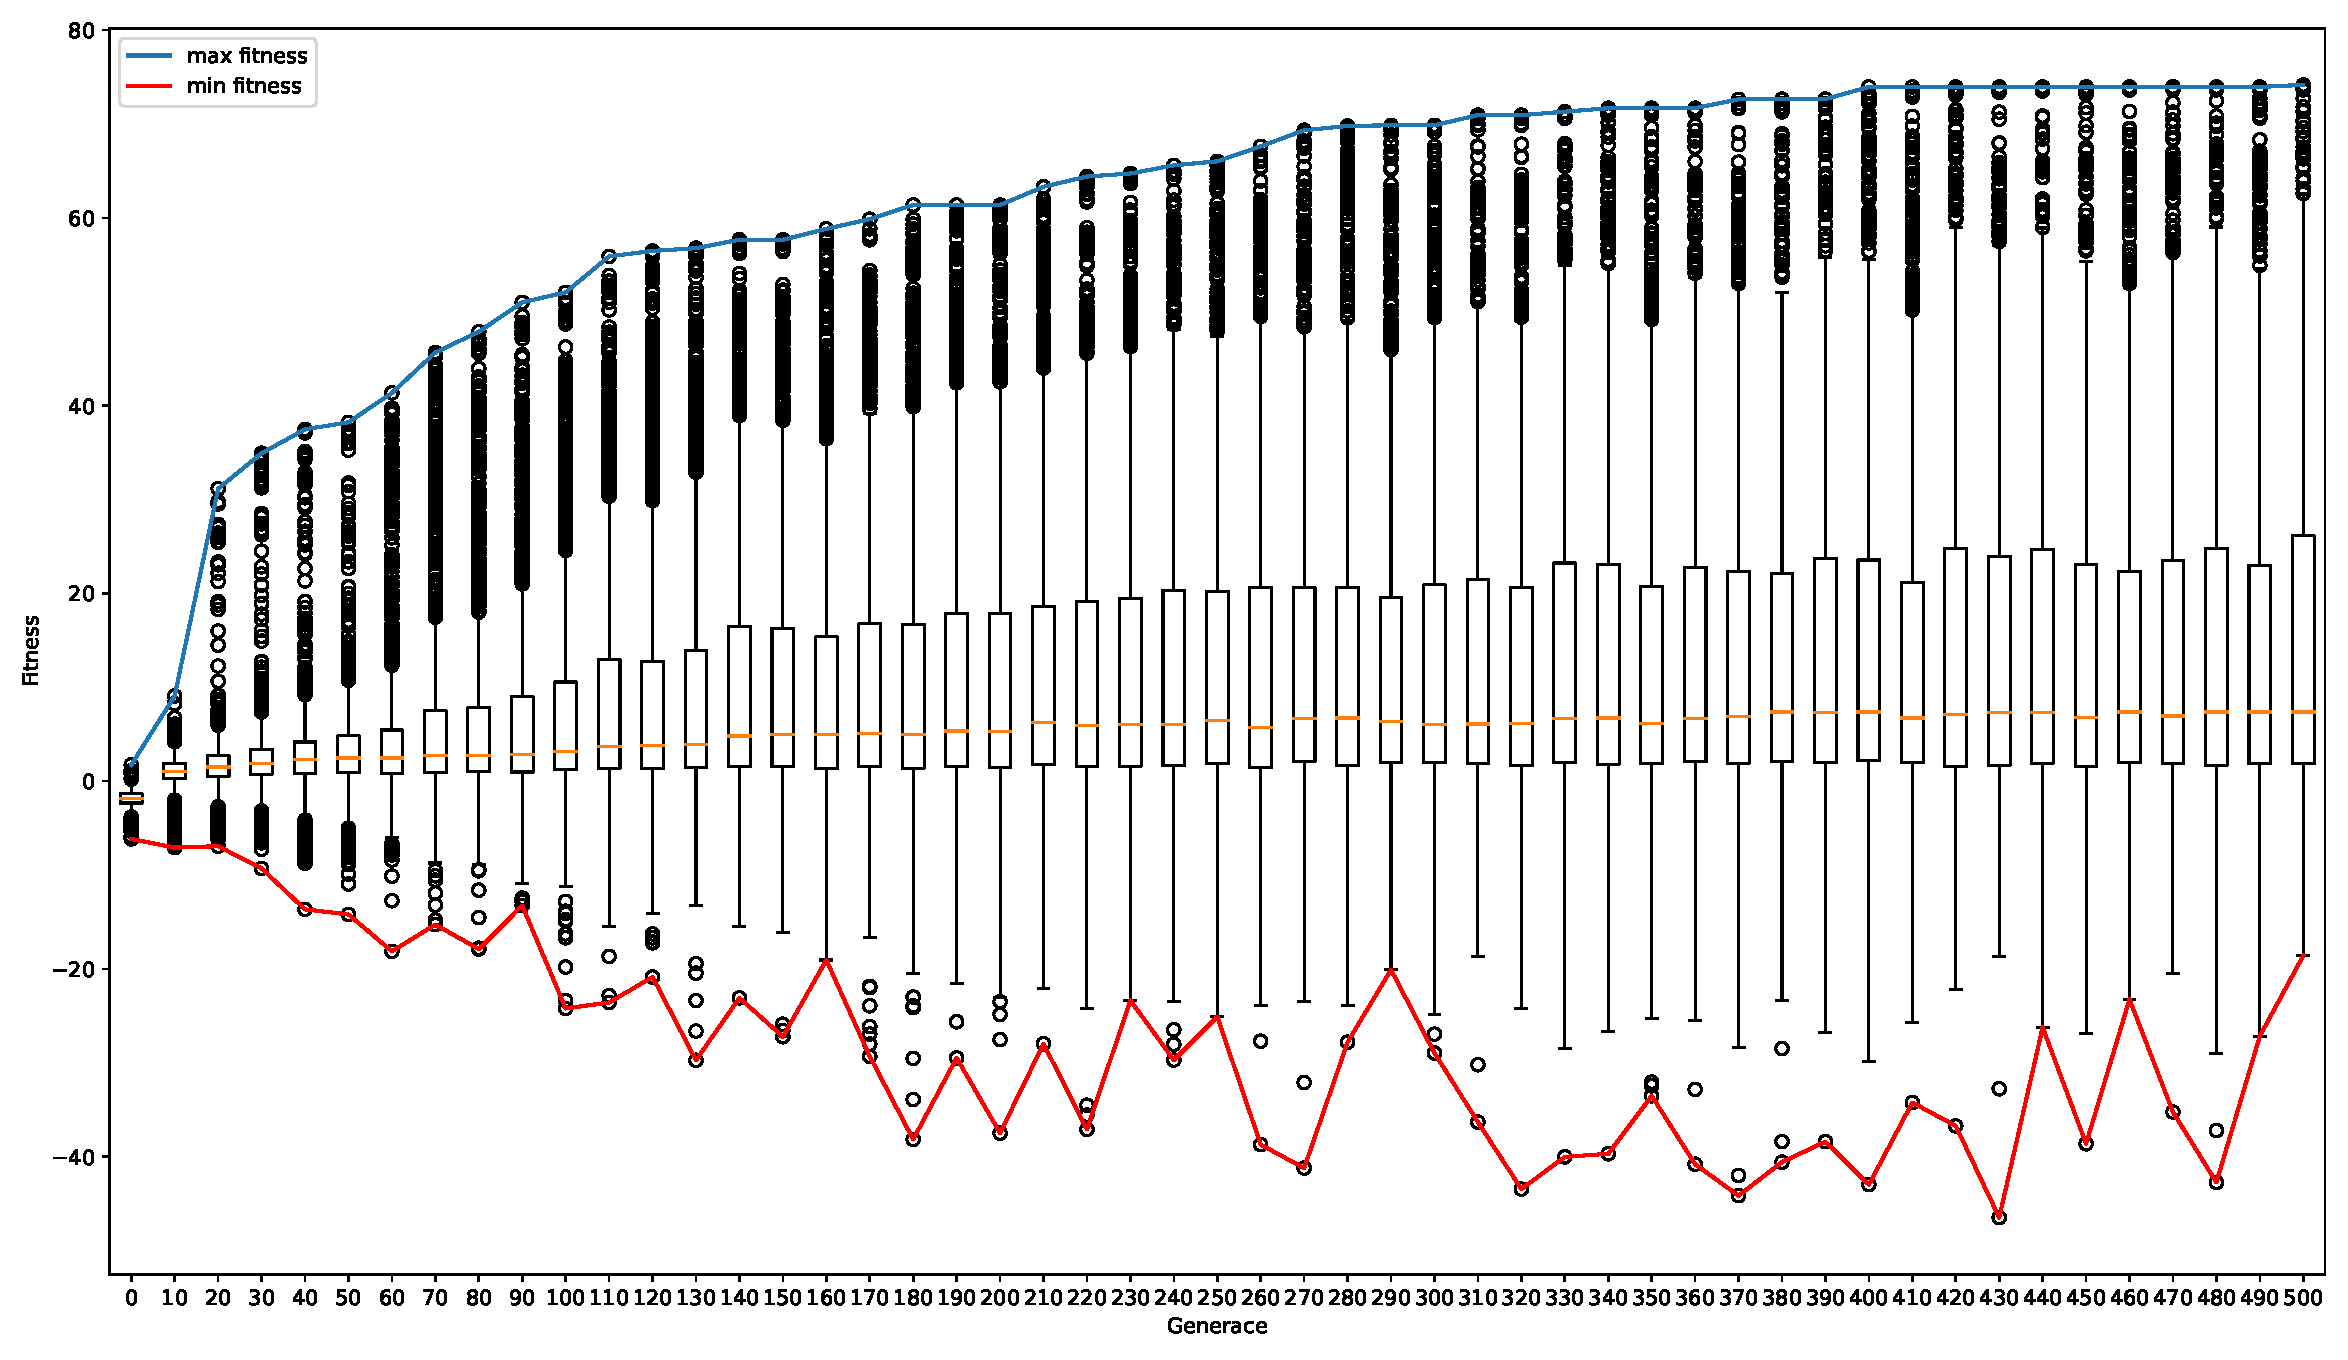
\includegraphics[width=1\textwidth]{../img/BIGexperiment1_TFS_10ticks.pdf}
    \caption{Velký experiment, 20 opakování algoritmu po 500 generacích, robot
    \emph{SpotLike}, agent \emph{TFSAgent}}
    \label{fig:exp_big}
\end{figure}

\paragraph{Krabicový graf}
Pro vizualizaci dat využíváme krabicový graf (boxplot). Tento graf vizualizuje
statistické rozložení dat pomocí kvartilů. Uprostřed se nachází \emph{krabice} (obdélník), který je
shora ohraničena 3. kvartilem a zespodu 1. kvartilem. Rozsah pokrytý
obdélníkem tedy obsahuje 50\% pozorovaných hodnot. Uvnitř \emph{krabice} se
nachází (v našich grafech oranžovou barvou) čára, naznačující hodnotu mediánu.
Dále krabicové grafy nad a pod střední \emph{krabicí} vykreslují tzv.
\emph{vousy}, což vizualizuje variabilitu dat nad 3. a pod 1. kvartilem. Dále
se v grafu mohou nacházet odlehlé body (\emph{outliers}), které jsou vykresleny
jako samostatné kroužky.

Grafy vznikají složením dat z průběhů fitness hodnot několika opakování daného
evolučního algoritmu. Jeden krabicový diagram pro danou generaci zobrazuje
rozložení hodnot fitness všech jedinců dané generace ze všech běhů. V grafu
\ref{fig:exp_big} je to celkem 2000 hodnot. V poslední generaci dále červené
značky označují hodnotu maximální fitness v jednotlivých bězích. 

V našich grafech pro přehlednost dále vykreslujeme hodnotu maximální (modrou
čarou) a minimální (červenou čarou) fitness v dané generaci.

Krabicový graf na obrázku \ref{fig:exp_big} zobrazuje vyhodnocení popsaného
velkého experimentu. Z grafu můžeme vidět, že největší růst fitness proběhl
přibližně v prvních 200 generacích. Optimalizace dále pokračovala a byla
schopná nacházet řešení s lepším hodnocením, ale pro účely vyhodnocování našich 
experimentů bude dostačující, když evoluci v tomto experimentu omezíme na 200
generací a algoritmus necháme vývoj pětkrát nezávisle zopakovat. To se nám
ukázalo jako dostatečné množství dat, které se podobá předvedenému velkému
experimentu a můžeme tak urychlit statistické vyhodnocení. 

Průběh předvedeného experimentu v obrázku \ref{fig:exp_big} trval přibližně 12
hodin i s využitím paralelizace ohodnocení jedinců mezi 12 vláken na výkonném
osobním počítači. Díky omezení dalších experimentů na menší počet generací a
opakování algoritmu jsme schopni na stejném systému následující experimenty
provést v řádech desítek minut.

\paragraph{První experiment}
Nejprve se pokusíme řízení robota \emph{SpotLike} (popsán v sekci
\ref{imp:robots.Spot}) vyvinout pomocí evolučního algoritmu, který kóduje
nastavení aktuátorů pomocí základních periodických funkcí (agent
\emph{SineFuncFullAgent} popisující tento algoritmus je popsán v implementaci v
sekci \ref{imp:gaAgents.sinefuncfullagent}). Každý aktuátor robota má v tomto
případě přiřazenou vlastní periodickou funkci a genotyp jedinců specifikuje
parametry těchto periodických funkcí (4 parametry pro každý kloub -- amplituda,
frekvence, $x$ a $y$ posun). Funkce jsou popsány rovnicí (\ref{sinefunc}) v
sekci implementace agentů.

Evoluční algoritmus běžel \textbf{200 generací} se \textbf{100} náhodně
inicializovanými jedinci. Pro vyhodnocení byl celý běh evolučního algoritmu
pětkrát opakován vždy s novou náhodně vygenerovanou počáteční populací.

\begin{figure}[!h]
    \centering
    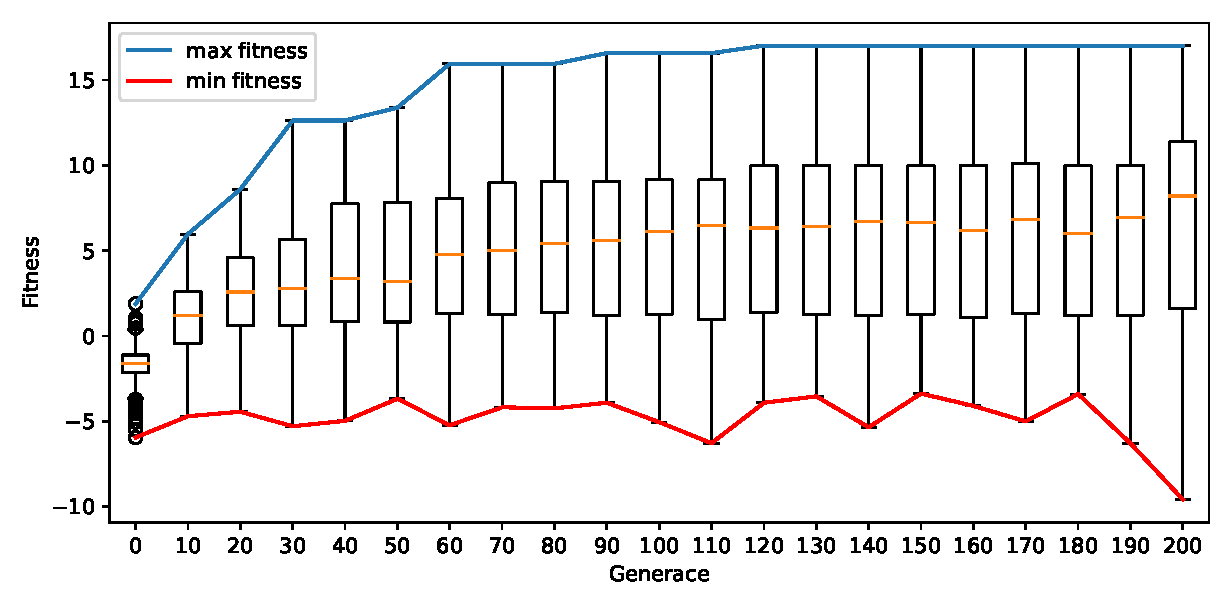
\includegraphics[width=1\textwidth]{../img/experiment1_Sine_10ticks.pdf}
    \caption{Vývoj fitness populace v experimentu se základním agentem\\
    \emph{SineFuncFullAgent} a robotem \emph{SpotLike}}
    \label{exp:first_sinefull}
\end{figure}

Graf na obrázku \ref{exp:first_sinefull} zobrazuje vývoj fitness
hodnot za běhu výše popsaného evolučního algoritmu. Data jsou vytvořena
kombinací záznamů o fitness hodnotách v dané generaci ze všech pěti nezávislých
běhů.

Z grafu se ukazuje, že tento přístup vývoje řízení dosáhl maximální hodnotu
fitness okolo 15 a populace na této hodnotě stagnovala a nebyla schopna většího
posunu.
%TODO: popsat units

\paragraph{Pokročilý agent}
Pro porovnání jsme zvolili pokročilého agenta \emph{TFSAgent}, který generuje
signály do aktuátorů pomocí omezených Fourierových řad (agent byl popsán v
sekci \ref{imp:gaAgents.TFSagent}). Tento agent je na úkor malého zvětšení
genotypu, oproti předchozímu agentovi schopný generovat mnohem komplexnější
periodické funkce popsané skládáním několika funkcí sinus.

Stejně jako v předchozím běhu, algoritmus běžel 200 generací se 100 jedinci a
byl opět pětkrát zopakován.

\begin{figure}[!h]
    \centering
    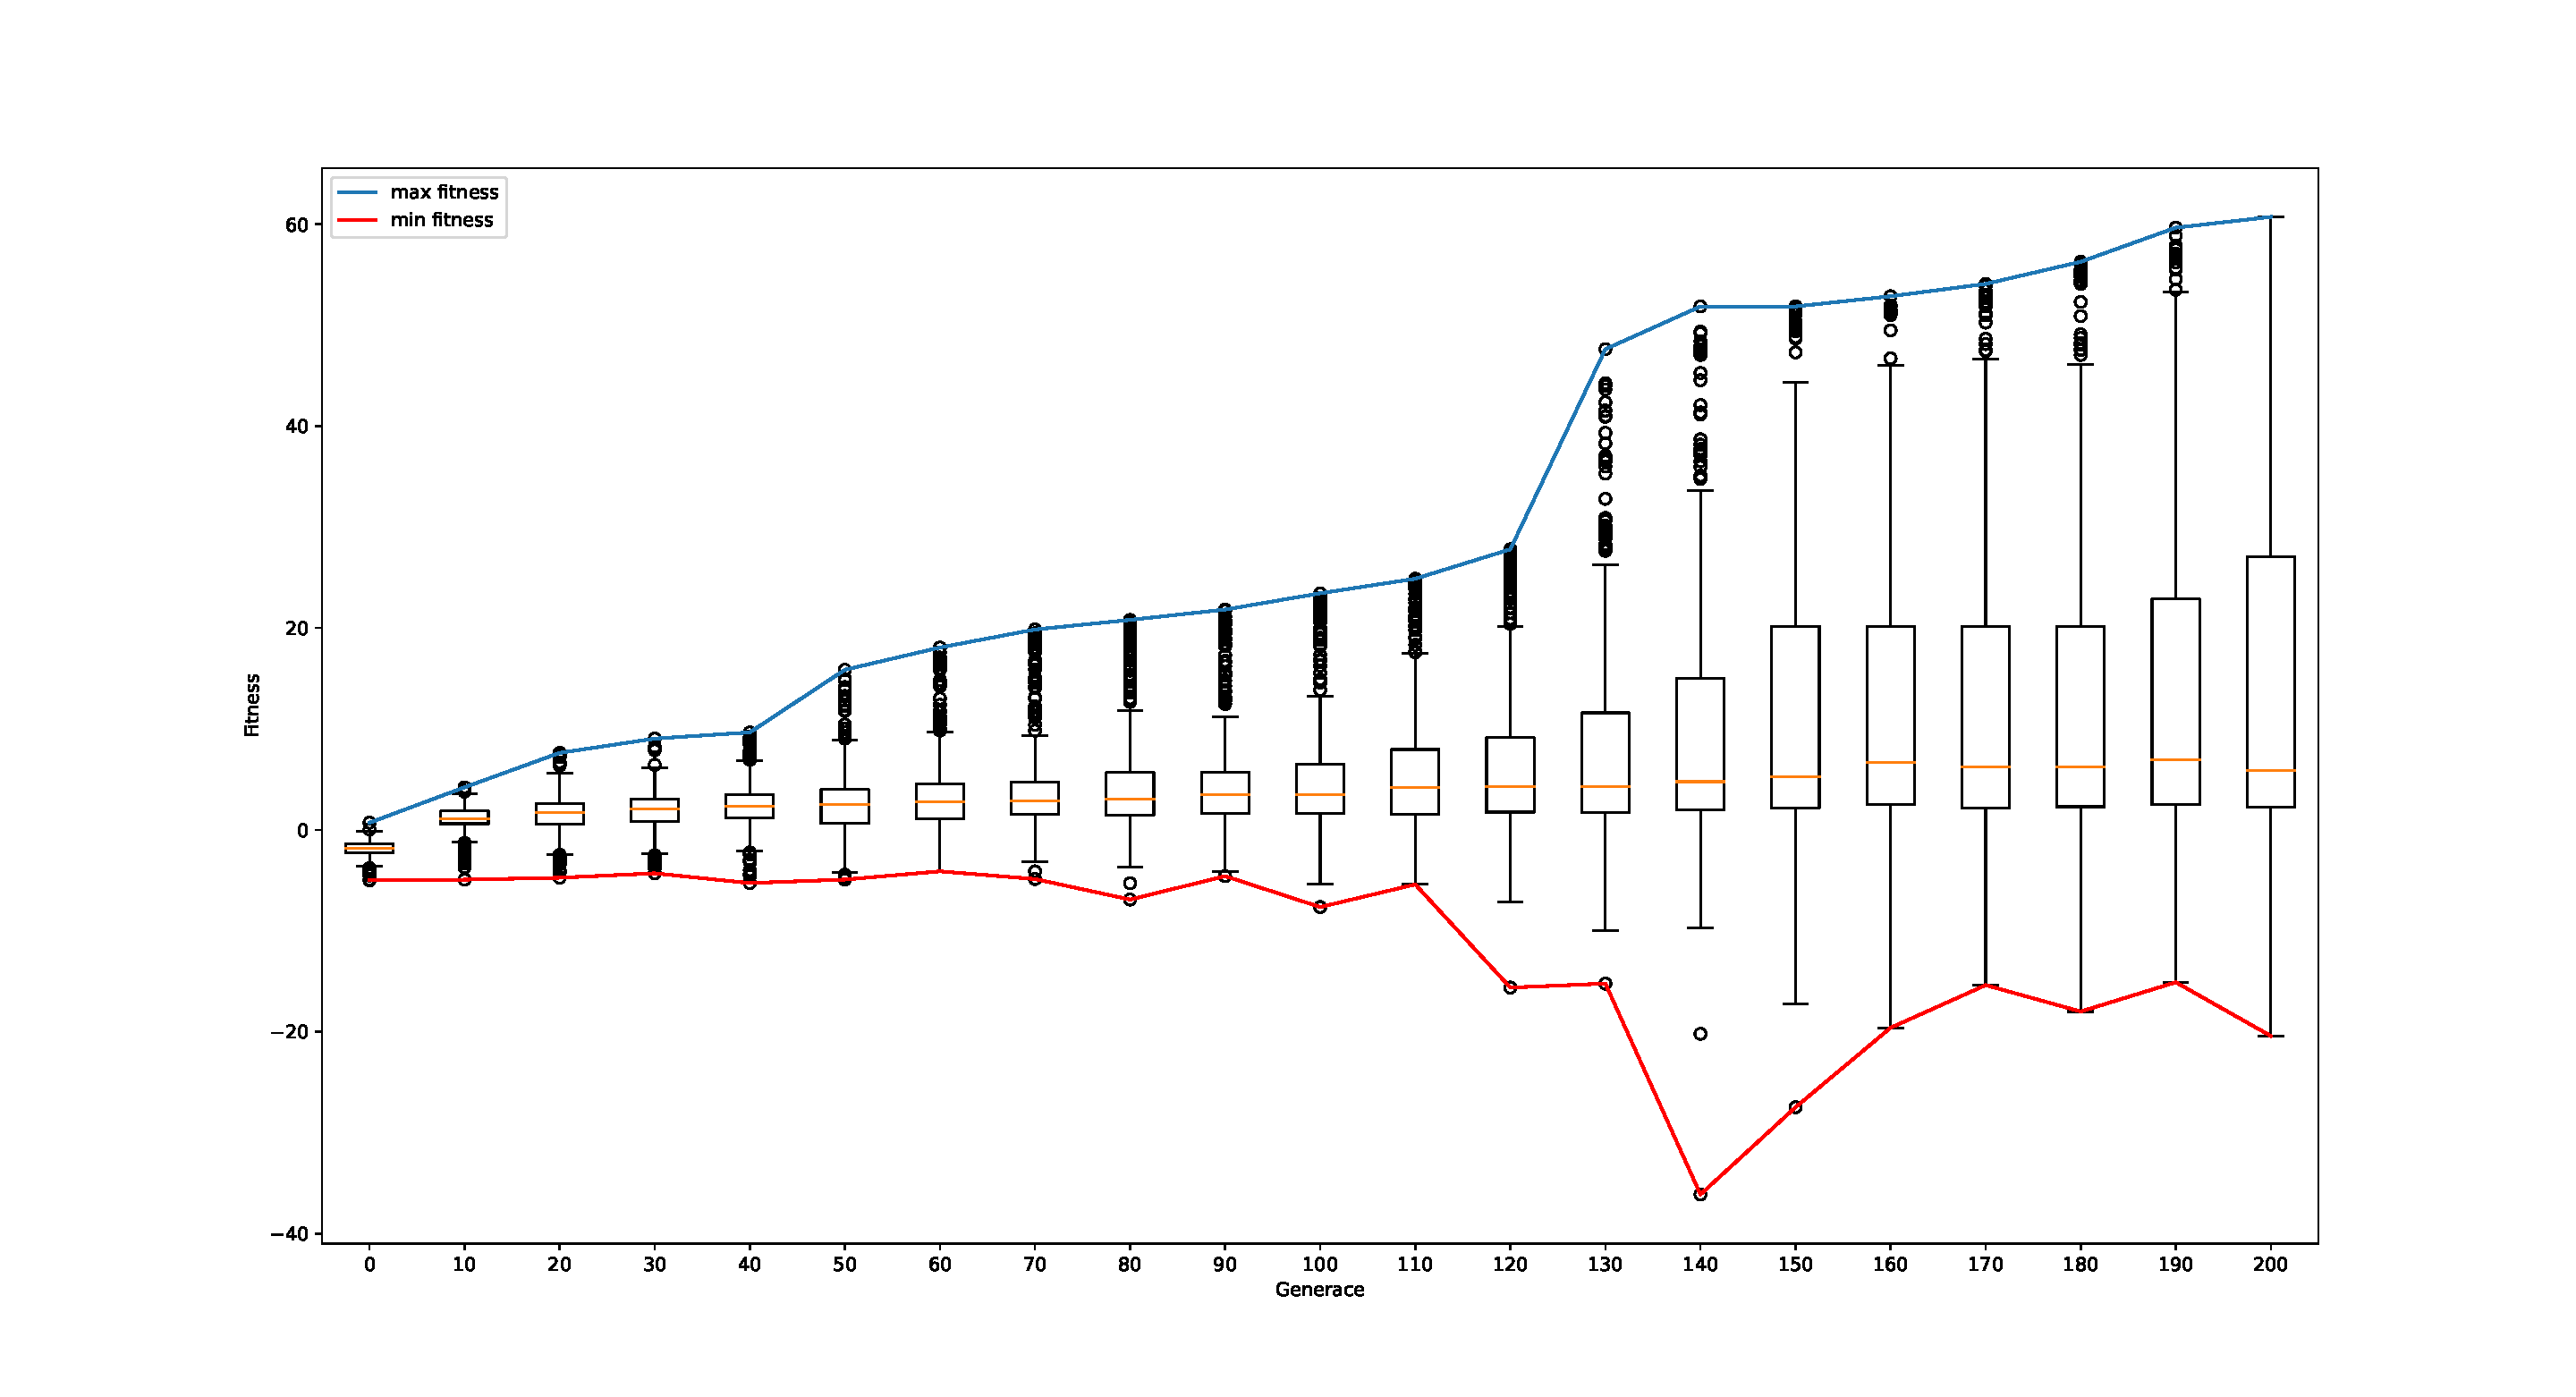
\includegraphics[width=1\textwidth]{../img/experiment1_TFS_10ticks.pdf}
    \caption{Vývoj fitness populace v experimentu s pokročilým agentem
    \emph{TFSAgent} a se stejným robotem \emph{SpotLike}}
    \label{exp:first_TFS}
\end{figure}

Graf \ref{exp:first_TFS} vývoje fitness hodnot z experimentu s pokročilým
agentem ukazuje, že tento agent již byl schopný vyvinout stabilní pohyb i pro
zadaného komplexního robota. Maximální fitness hodnota, které při vývoji agent
dosáhl, se pohybovala okolo 60. Zároveň podle krabicového grafu vidíme, že
poměrně velká část populace byla schopná dosáhnout výsledků, přesahující
nejlepší výsledky jednoduššího agenta.

\paragraph{}
Z experimentů jsme zároveň dostali i nejlepšího jedince z poslední generace
evolučního algoritmu. Jelikož naše simulované fyzikální prostředí je
deterministické, můžeme řešení nejlepšího jedince zpětně vizualizovat.

Ruční kontrolou těchto výsledků jsme dále zjistili, že pouze část (dva z pěti
běhů) dosáhly takového pohybu, který bychom od robota této morfologie
očekávali. Tělo v robota v těchto případech (až na menší odchylky) směřovalo
rovně, způsobem připomínající chůzi čtyřnohých zvířat podobné morfologie. Zbylé
běhy vyvinuly stabilní, ale ne zcela estetickou chůzi. Roboti se v těchto
případech posouvali stranou využitím většího rozsahu v rotaci
(\emph{kyčelních}) kloubů. Pravděpodobně kvůli lepší stabilitě robota.

Osobně si myslím, že vývoj estetického pohybu pro tohoto robota je s malou
úpravou hodnotící funkce možný. Ta by například mohla penalizovat rotaci těla
od požadovaného směru pohybu. Chůze stranou je kvůli rozsahu (\emph{kyčelních})
kloubů (hlavně v ose délky těla robota) mnohem snazší na vyvinutí a tak tento
způsob chůze tvoří silné lokální optimum. Agenti velmi rychle konvergují ke
způsobům chůze, které jsou stabilní, což jim navyšuje šanci urazit větší
vzdálenost bez pádu. Chůze stranou je oproti vratké chůzi rovně mnohem
stabilnější. Navržená jednoduchá úprava hodnotící funkce by měla být schopna
toto lokální optimum penalizovat a tedy přinutit estetičtější pohyb.

\paragraph{}
Ve srovnání s předchozími pokusy jsme se pomocí stejných agentů snažili
vyvinout řízení jednoduššího robota označeného jako \emph{Ant} (zobrazeného na
obrázku \ref{fig:robot:ant}, blíže popsán v implementaci v sekci
\ref{imp:robots.Ant}). Můžeme ho brát jako jednoduššího, protože obsahuje menší
počet kloubů (8 stupňů volnosti) v porovnání s robotem \emph{SpotLike}. Zároveň
jeho morfologie umožňuje snazší pohyb všemi směry s menším rizikem pádu.

\begin{figure}[!htb]
    \centering
    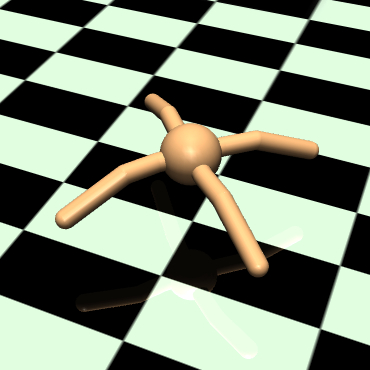
\includegraphics[width=0.4\textwidth]{../img/crop_Ant-v3.jpg}
    \caption{Robot \emph{AntV3}}
    \label{fig:robot:ant}
\end{figure}

Řízení jsme vyvíjeli pomocí agentů se stejnými parametry jako v případě s
pokročilým robotem. Celý běh byl opět pro statistické vyhodnocení pětkrát
opakován se stejnou velikostí náhodně vygenerované populace (\textbf{100
jedinců}). Jelikož jsme kvůli menšímu počtu stupňů volnosti očekávali schopnost
agentů vyvinout řízení rychleji, zkrátili jsme délku evoluce na \textbf{100
generací}.

\begin{figure}[h!]
    \centering
    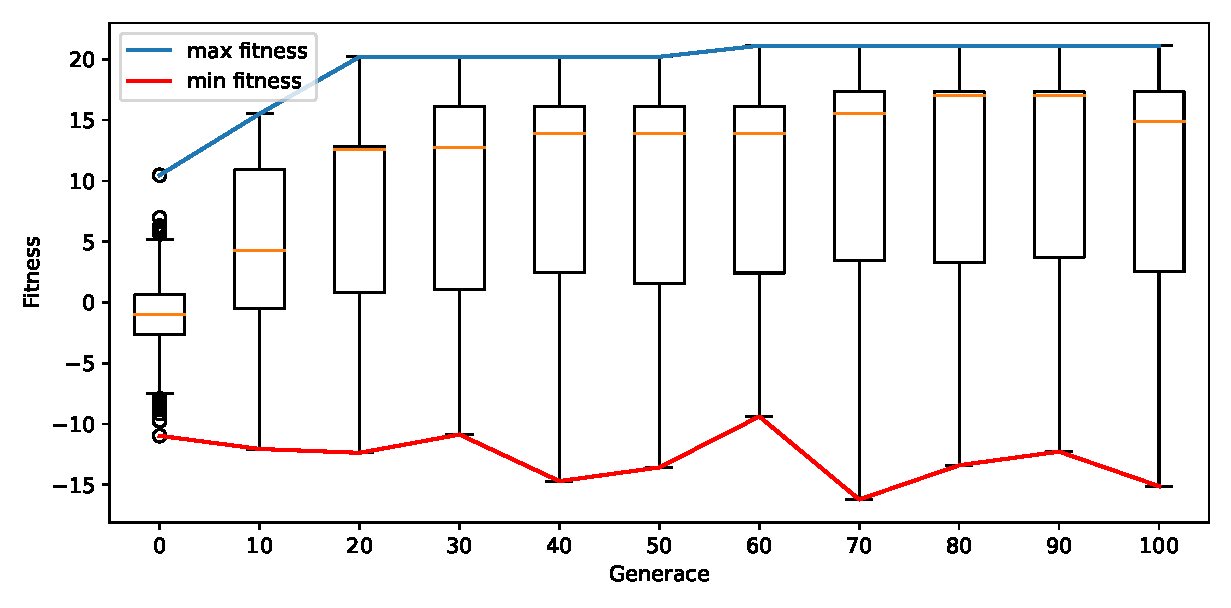
\includegraphics[width=1\textwidth]{../img/experiment1_2_Sine_10ticks.pdf}
    \caption{Vývoj fitness populace se základním agentem
    \emph{SineFuncHalfAgent} a jednodušším robotem \emph{AntV3}}
    \label{exp:first2_sinefull}
\end{figure}
\begin{figure}[h!]
    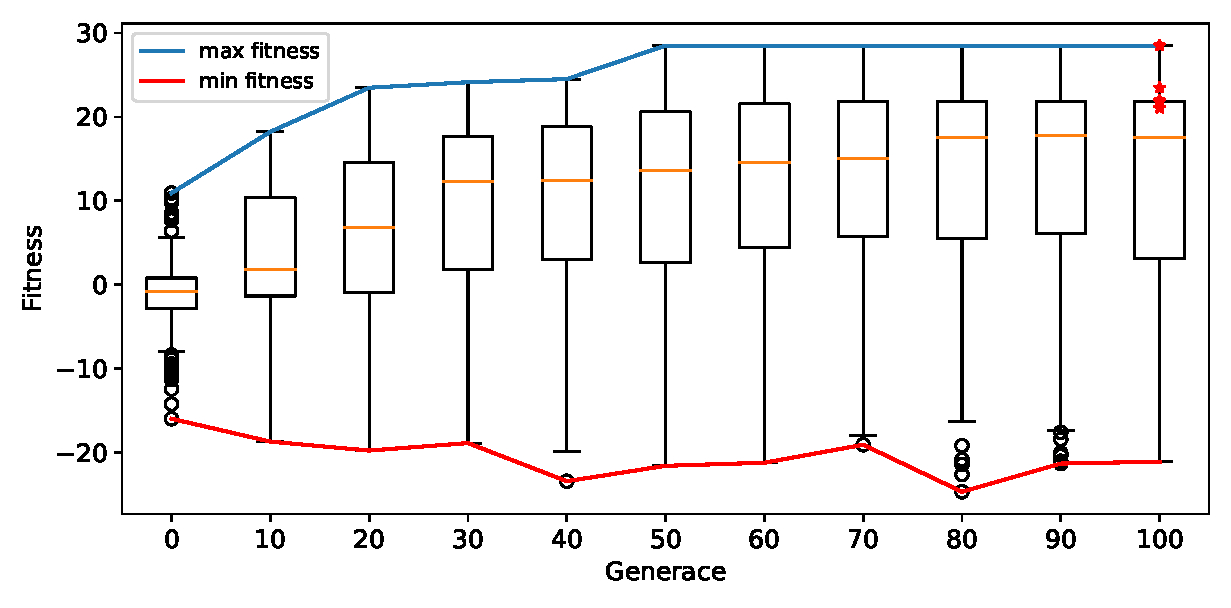
\includegraphics[width=1\textwidth]{../img/experiment1_2_TFS_10ticks.pdf}
    \caption{Vývoj fitness populace s pokročilým agentem \emph{TFSAgent} a
    jednodušším robotem \emph{AntV3}}
    \label{exp:first2_TFS}
\end{figure}

Z vývoje fitness (v grafu \ref{exp:first2_sinefull} a \ref{exp:first2_TFS})
můžeme pozorovat, že oba agenti byli schopní u tohoto jednoduššího robota
dosáhnout přijatelných výsledků i s omezeným počtem generací. Přijatelné
výsledky jsou částečně podpořeny faktem, že i náhodné konfigurace mají dobrou
šanci tohoto robota rozpohybovat v požadovaném směru a tedy již velmi brzy
získat dobré ohodnocení. To se zároveň projevuje i na minimální fitness. Pro
tohoto robota je totiž stejně jednoduché dostat takovou konfiguraci aktuátorů,
které ho rozpohybují v opačném směru (jedinec z definice hodnotící funkce
obdrží záporné ohodnocení).

\section{Vývoj řízení a morfologie robotů} \label{exp2}

V této sekci předvedeme dva další typy experimentů, které naše knihovna
podporuje -- simultánní vývoj (v sekci \ref{exp2:para_evo}) a oddělený
vývoj (v sekci \ref{exp2:split_evo}) řízení a morfologie.

Tyto experimenty se od předchozích liší tím, že evolučnímu algoritmu povolíme
vyvíjet i zvolené části těla robota. To teoreticky umožní z těla původního
robota vyvinout optimálnější morfologii pro zadaný problém.

Vývoj těla je implementací umožněn díky speciálním značkám v XML konfiguračních
souborech (popsaných v konfiguraci vlastního robota v sekci \ref{imp:robots}).

\subsection{Simultánní vývoj řízení a morfologie} \label{exp2:para_evo}

V prvním příkladu předvedeme experiment, ve kterém umožníme evolučnímu
algoritmu vyvíjet zároveň řízení i morfologii robota. Tento experiment by
teoreticky mohl pomáhat v optimalizaci morfologie robotů za hranici
představivosti jejich autorů. 

Pro vývoj morfologie volíme při inicializaci agenta \emph{masku} těla
robota (popsána v parametru \texttt{body\_part\_mask} v sekci
\ref{imp:gaAgents}). Tato maska popisuje, které části těla mají při vývoji
zůstat beze změny a zároveň určuje povolené rozsahy hodnot pro části
těla otevřených pro evoluční vývoj.

Kvalita jedinců byla v tomto experimentu hodnocena stejně jako v předchozích
experimentech. Cílem pro jedince je tedy dojít co nejdále v určeném směru.
Přesný výpočet fitness je popsán rovnicí (\ref{fitness_calc}). 

Pro experiment jsme zvolili robota \emph{AntV3} (popsán v implementaci v sekci
\ref{imp:robots.Ant}). Tento typ experimentů je ale samozřejmě povolen pro
libovolného robota, který umožňující evoluční vývoj alespoň jedné části těla.

\paragraph{Vývoj robota \emph{AntV3}}
Jak bylo řečeno v této ukázce jsme zvolili robota \emph{AntV3}. Pro vývoj
robota byl využit agent \emph{SineFuncHalfAgent} (popsaného v sekci
\ref{imp:gaAgents.sinefunchalfagent}). \emph{AntV3} je robot se složitější
morfologií končetin a z tohoto důvodu ho vybíráme pro demonstraci tohoto typu
vývoje.

Tento experiment je nakonfigurovaný v modulu \emph{experiment\_setter} pod
názvem \texttt{exp2\_body\_para}. Pro evoluční algoritmus byla zvolena velikost
populace na \textbf{150 jedinců} (větší velikost populace zvolena kvůli
rozšíření prohledávaného prostoru, ve kterém evoluce hledá optimální řešení) a
evoluci byl umožněn vývoj po \textbf{200 generací}. Zároveň byl zvolen povolený
rozsah délek částí končetin pro vývoj. Robot \emph{AntV3} (na obrázku
\ref{fig:robot:ant}, popsán v sekci \ref{imp:robots.Ant}) má 4 končetiny
složené ze dvou částí -- pro jednoduchost je označme jako \emph{stehno} a
\emph{lýtko}. V základní konfiguraci je délka \emph{stehna} pro tohoto robota
$0.2$ (pro vývoj zvolen rozsah mezi $0.1$ a $0.5$) a délka \emph{lýtka} je
$0.4$ (pro vývoj umožníme rozsah mezi $0.15$ a $0.5$). Délka libovolné části těla je při
vývoji nezávislá na ostatních.

\begin{figure}[h!]
    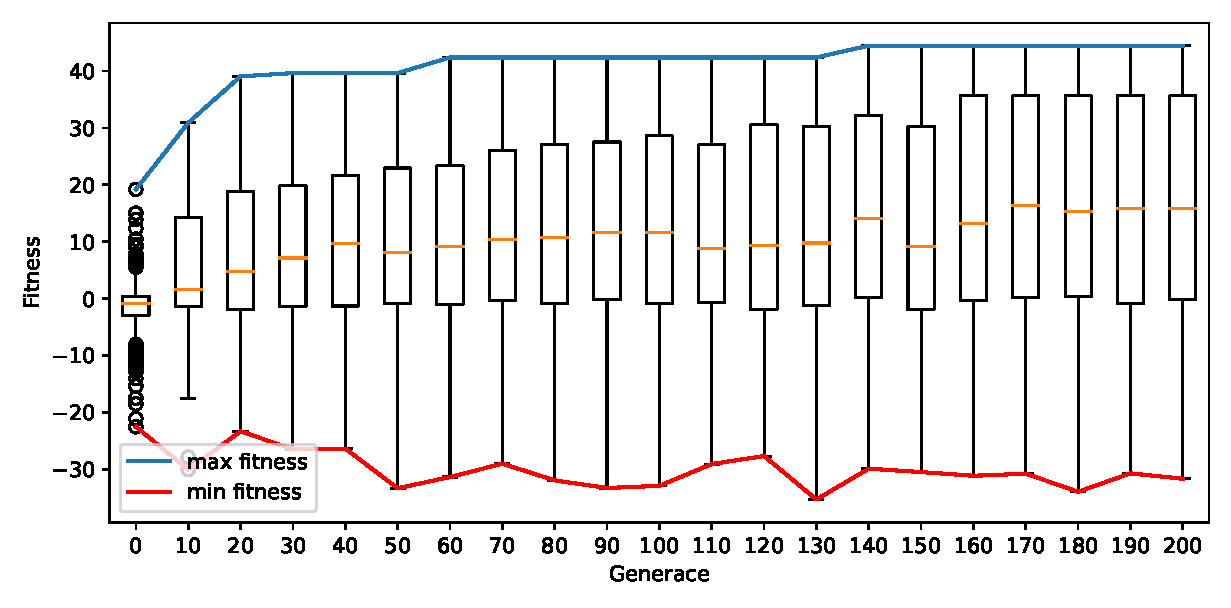
\includegraphics[width=1\textwidth]{../img/experiment2_para_10ticks.pdf}
    \caption{Vývoj fitness populace při současném vývoji řízení a morfologie s
    agentem \emph{SineFuncHalfAgent} a robotem \emph{AntV3}}
    \label{exp:exp2_para}
\end{figure}

Z grafu na obrázku \ref{exp:exp2_para} můžeme pozorovat, že tento typ vývoje
zvládl stabilně produkovat vyšší fitness hodnoty než srovnatelný předchozí
experiment (využívající stejného agenta i robota) nevyužívající vývoje
morfologie (graf na obrázku \ref{exp:first2_TFS}). Můžeme tedy odhadovat, že
mohou existovat optimálnější konfigurace končetin tohoto robota, než jaká je
výchozí.

\begin{figure}[h!]
    \centering
    \begin{minipage}{0.5\textwidth}
        \centering
        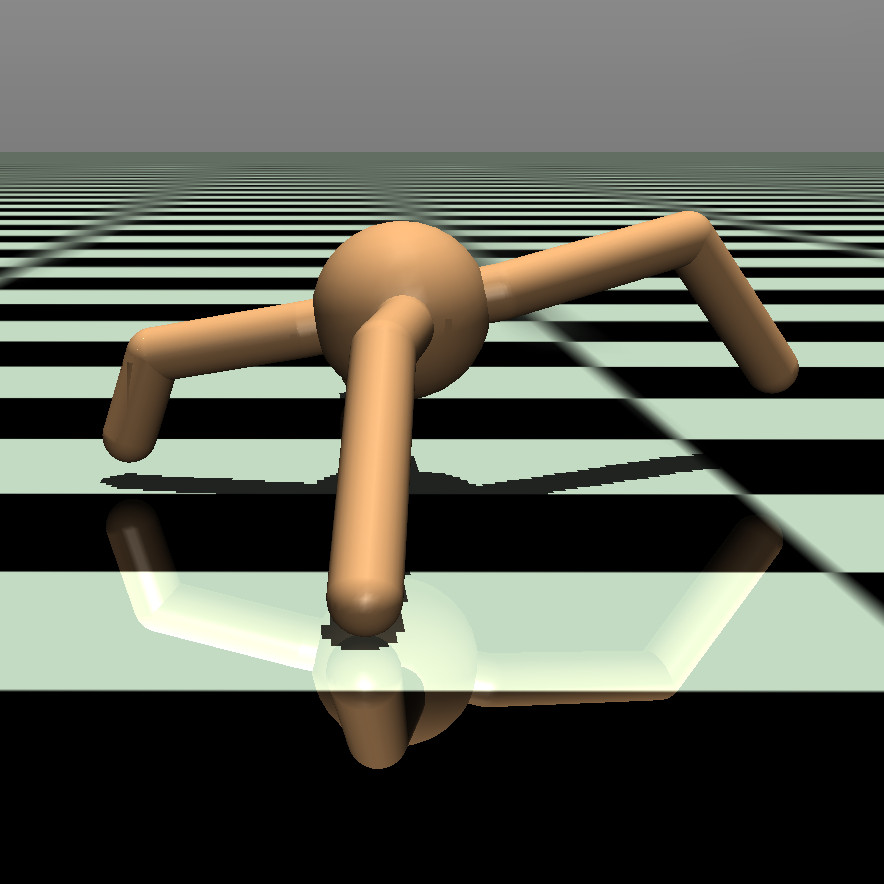
\includegraphics[width=0.75\textwidth]{../img/crop_exp2_para_side1.jpg}
    \end{minipage}%
    \begin{minipage}{0.5\textwidth}
        \centering
        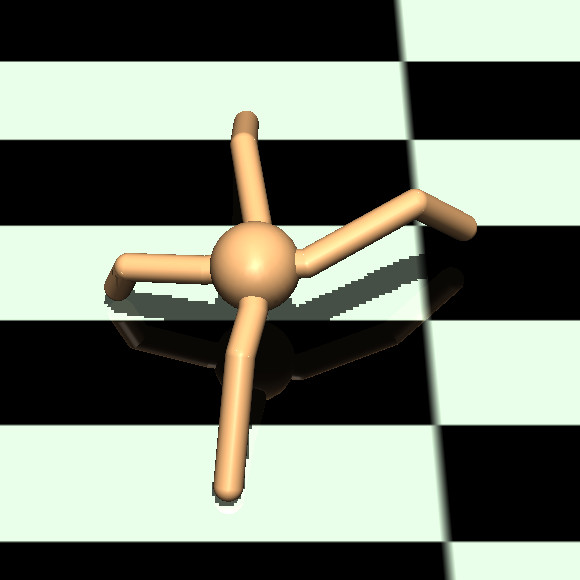
\includegraphics[width=0.75\textwidth]{../img/crop_exp2_para_top1.jpg}
    \end{minipage}
    \caption{Příklad z výsledků současného vývoje řízení a morfologie robota
    \emph{AntV3}}
    \label{fig:exp2_para_body_show}
\end{figure}

Díky možnosti přehrávání nejlepších řešení jednotlivých běhů algoritmu můžeme
zároveň prozkoumat, k jakým konfiguracím vývoj dospěl. Ukázalo se, že vývoj
dospěl buď k robotům s velmi dlouhými končetinami, nebo (jak je na obrázcích
\ref{fig:exp2_para_body_show}) k robotům s několika dlouhými
(\emph{odrazovými}) končetinami a jednou kratší končetinou (sloužící jako
\emph{kormidlo}). 

Obrázky \ref{fig:exp2_para_body_show} ukazují nejúspěšnějšího robota z
předvedeného experimentu, který je schopný své tělo díky kratší zadní noze
naklonit, a je tak schopný poměrně rychle skákat vpřed.

\subsection{Oddělený vývoj řízení a morfologie} \label{exp2:split_evo}
V tomto experimentu předvedeme druhý typ vývoje řízení a morfologie robota a to
oddělený vývoj. V tomto typu evolučního vývoje se nejprve provede vývoj řízení
robota s výchozí morfologií. Následně se vývoj řízení zafixuje ve stavu
populace z poslední generace a začne druhá část vývoje, ve kterém se vyvíjí
pouze morfologie robota.

Jedinci tak dostanou možnost nejprve vyvinout samotný pohyb (jak tomu bylo v
prvním experimentu) a následně evolučním vývojem optimalizovat tělo pro
specifický pohyb. Tímto přístupem by teoreticky jedinci měli být schopni
dosáhnout lepších výsledků, než při vývoji samotného řízení.

Pro tento experiment jsme zvolili stejného robota (s totožnými rozsahy
velikostí končetin) a stejného agenta jako v předchozím experimentu.
Konfigurace experimentu je v modulu \emph{experiment\_setter} pod
názvem \texttt{exp2\_body\_serial}. Evoluční algoritmus běžel nejprve 100
generací, při kterých se vyvíjelo řízení robota a následně 100 generací pro
vývoj morfologie.

\begin{figure}[h!]
    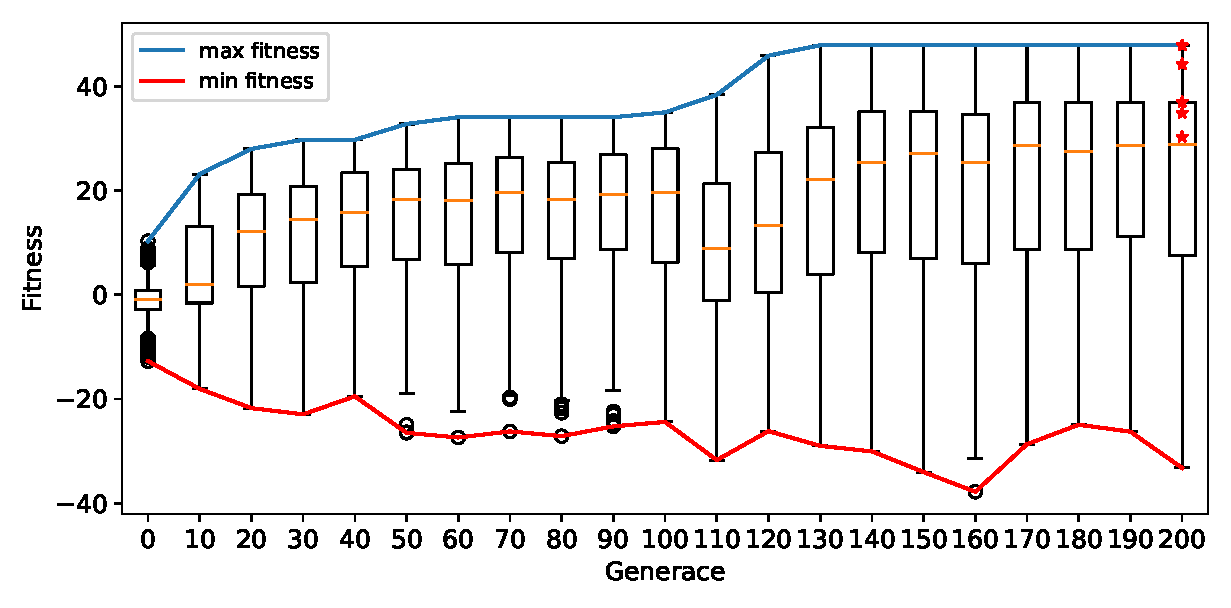
\includegraphics[width=1\textwidth]{../img/experiment2_serial_10ticks.pdf}
    \caption{Vývoj fitness populace při odděleném vývoji řízení a morfologie
    s agentem \emph{SineFuncHalfAgent} a robota \emph{AntV3}}
    \label{exp:exp2_serial}
\end{figure}

V grafu na obrázku \ref{exp:exp2_serial} můžeme pozorovat vývoj fitness v
jednotlivých generacích. Můžeme vidět, že po 100. generaci přišel malý pokles
průměrných fitness hodnot, což bylo zapříčiněno začátkem vývoje morfologie
robota. Ten začíná vygenerováním zcela náhodných konfigurací těla robota (v
povoleném rozsahu délek končetin), a tedy může chvilkově vést k horším
výsledkům. Časem ale vidíme, že evoluce byla schopná optimalizovat tělo robota
pro již vyvinutý pohyb a tak celkově vylepšit výsledky jedinců.

\begin{figure}[h!]
    \centering
    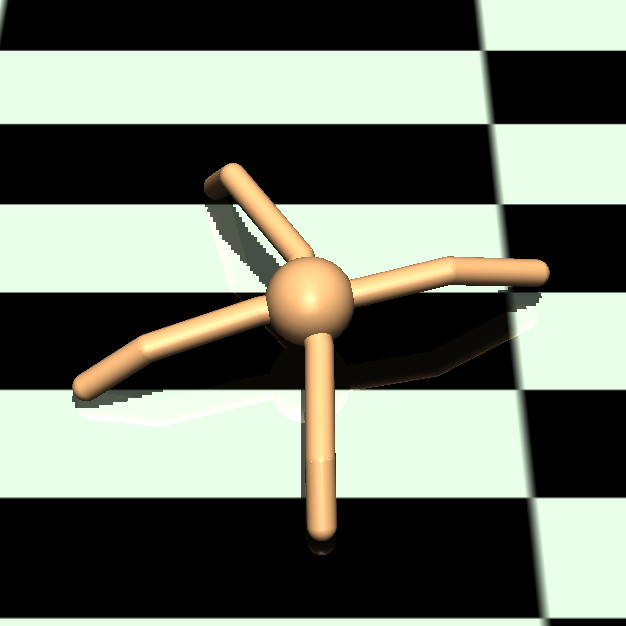
\includegraphics[width=0.4\textwidth]{../img/crop_exp2_serial_top1.jpg}
    \caption{Příklad z výsledků odděleného vývoje řízení a morfologie robota
    \emph{AntV3}}
    \label{fig:exp2_serial_body_show}
\end{figure}

Na obrázku \ref{fig:exp2_serial_body_show} můžeme vidět nejlepšího jedince z
experimentu s odděleným vývojem řízení a morfologie. Jedná se zároveň o dobrý
příklad morfologie, ke které se řešení často blížila. Pro tento typ pohybu se 
robotům hodilo mít mnohem delší části končetin vedoucí přímo od těla
(\emph{stehno}), které svým pohybem jsou schopny posunout robota dále a tak
optimalizovat uraženou vzdálenost.

% \section{Diskuze výsledků}
